
\chapter{Developer documentation}

\section{Algorithms and data structures used}

\subsection{The representation of a metaprogram}

%Mihalicza: page 69
C++ template metaprogramming can be seen as a form of purely functional
programming.\cite{mihalicza-phd} In functional programming a program's main
components are the functions. In metaprogramming, functions are represented by
so called metafunctions. Metafunctions are basically templated structs or
classes, which get their parameters as template parameters, and return values
by defining member types or compile time constants based on the template
parameters.

For a specific metaprogram, Metadebugger represents only the metaprogram's call
graph. For example instantiating \verb|int_<fib<5>::value>| would be
represented by the following graph in Metadebugger:

\includegraphics[width=\textwidth]{img/fib5_call_graph.eps}

It can be seen from the above graphic, that the graph vertices represent types,
and edges represent instantiation events. A type can instantiate multiple
types, and a type can be referenced from multiple places. The first reference
to a type will be a TempateInstantiation event (as it is instantiated for the
first time by the compiler). The following references will reuse the already
created type, so those become Memoization events.

\subsection{Graph filtering} \label{graph-filtering}

The underlying C++ compiler emits a lot of instantiation events which don't
have real value to the user. These events need to be filtered out from the
graph for better user experience. The edges which represent these events are
not physically taken out from graph, only an edge property flag is set to
disable the edge. Algorithms which traverse the graph will of course have to
check this flag to operate only on the interesting part of the graph.

The decision to only use a flag instead of modifying the graph has the
following properties:

\begin{itemize}
    \item
        Faster filtering process, since the internal vectors used to represent
        the graph are not touched.
    \item
        Uses more memory, since memory used by unused data are not freed back
        to the operating system.
    \item
        Not currently implemented, but these unused parts of the graph can be
        enabled for the advanced users, if they're interested.
    \item
        In boost's graph implementation, \verb|vertex_descriptor|
        objects used to refer to vertices of the graph are unsigned integers.
        The documentation promises, that these \verb|vertex_descriptor|
        start from 0 and go up from there for every vertex added to the graph.
        The algorithms in Metadebugger relies heavily on this handy property.
        Removing vertices from the graph would break this continous indexing.
\end{itemize}

The filtering process takes multiple stages. The filter algorithm starts out
with a graph, where all edges are enabled.

\begin{enumerate}
    \item
        Disable all edges. This is useful because the following stages become
        simpler.
    \item
        Enable edges going from the root vertex for which the
        \verb|point_of_instantiation| edge property matches the currently
        entered line. This is to filter out instantiation subtrees, which were
        not initiated by the type entered by the user.
    \item
        Now a depth first traversal is done from the root vertex going only on
        the edges we enabled in the previous section. For every new vertex the
        traversal encounters, the algorithm enables all out edges, and
        continues the traversal through these edges.
    \item
        Clang generates a TemplateInstantiation and a Memoization event for the
        result type. Disable the Memoization one. In this process, the name of
        the vertex pointed by these two edges is trimmed too, so the
        \verb|metashell::wrap| wrapper doesn't clutter the result.
    \item
        Clang sometimes triggers multiple Memoization events for the same type
        instantiated from a single type, and thus equivalent parallel edges
        appear in the graph. Since the user doesn't get any useful information
        about how many times Clang internally checked a type instantiation,
        these get filtered out as well.
\end{enumerate}

\subsection{Forwardtrace}

When at some point the user wants to see what will happen in the future with
the current type it is the eaisest to issue a forwardtrace command. Here is
what the forwardtrace looks like from the very beginning of the evaluation of
\verb|int_<fib<5>::value|:

\bigskip

% TODO this on a white background
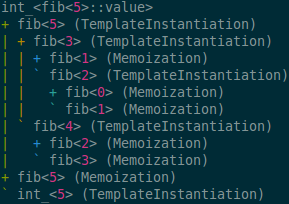
\includegraphics[width=0.5\textwidth]{img/fib5_ft.eps}

The algorithm which prints this is basically a depth first traversal printing
a line every time it visits a vertex. The algorithm is iterative and thus keeps
track of the edges it has to visit in a stack. In addition it also keeps track
of the current depth of the traversal in the stack, so the depth of the
identation is known when printing a line.

For better readability, it is also required to know for every depth less than
the current depth if the algorithm should print a \verb$'|'$ or not. This
is achieved by having a vector of counters from 0 to the current depth. Each
element in the vector counts how many elements are there in the stack with that
particular depth. For every depth, the algorithm prints \verb$'|'$ when
this counter is greater than 0.

\subsection{Stepping}

The algorithm for basic stepping is very similiar to forwardtrace: in it's core
it is also a depth first traversal of the underlying call graph. There are two
other extra things step has to be able to do:

\begin{enumerate}
    \item
        Stop at any point in the traversal, so the user can inspect the current
        state of the metaprogram.
    \item
        Going backwards in the traversal. This happens, when the user calls the
        step command with a negative argument.
\end{enumerate}

Stopping at any point is achieved by creating a \verb$state_t$ structure
which describes the current state of the metaprogram. It was put in the
metaprogram class' scope, and a \verb$void metaprogram::step()$ function
was created which does a single iteration of the depth first traversal by
updating the state structure. The \verb$state_t$ struct and the step
function:

\includecode{src/metaprogram_state_t.hpp}

The other extra feature of stepping is going backwards. A
\verb$void metaprogram::step_back()$ functions was created which also
updates the state struct, but does the opposite of \verb$step()$. This
means, that if \verb$step()$ was called from state A and resulted in state
B, then calling \verb$step_back()$ from state B will result in state A.
The two endpoint states (when nothing has been discovered and when every
reachable vertex were discovered) are exceptions from this rule.

When step is executing, it marks the changes it made into the state into a
\verb$rollback_t$ structure and pushes them onto a stack:

\includecode{src/metaprogram_rollback_t.hpp}

\verb$step_back()$ simply picks pops the top element from the stack, and
restores the state change the last \verb$step()$ did, based on the
rollback structure.

% TODO actual algorithms and state diagram

\subsection{Command matching}

Users of any software will want to do a particular task with less and less
effort as they get more experience with the tool. For a command line tool like
Metadebugger, this need basically boils down to typing as few characters as
possible.

To aid this, an algorithm similar to gdb's command matching was implemented.

If the user enters a prefix of a command which uniquely identifies the command
(so there is no other command with that same prefix), than that command should
be executed. In Metadebugger some commands also have aliases (for example, a
shortened alias for the command \verb$"backtrace"$ is \verb$"bt"$). The
the entered command should also be accepted when it is not a prefix for a
unique command, but all possible candidate commands are aliases for the same
command. For example the input \verb$"b"$ should be accepted as a command
for backtrace, even though it is not a unique prefix.

Pseudocode for the algorithm:

\includecode{src/command_matching.cpp}

\pagebreak

\section{Class hierarchy}

Here is the class diagram for the main classes that have something to do with
Metadebugger.

\begin{figure}[H]
\centering
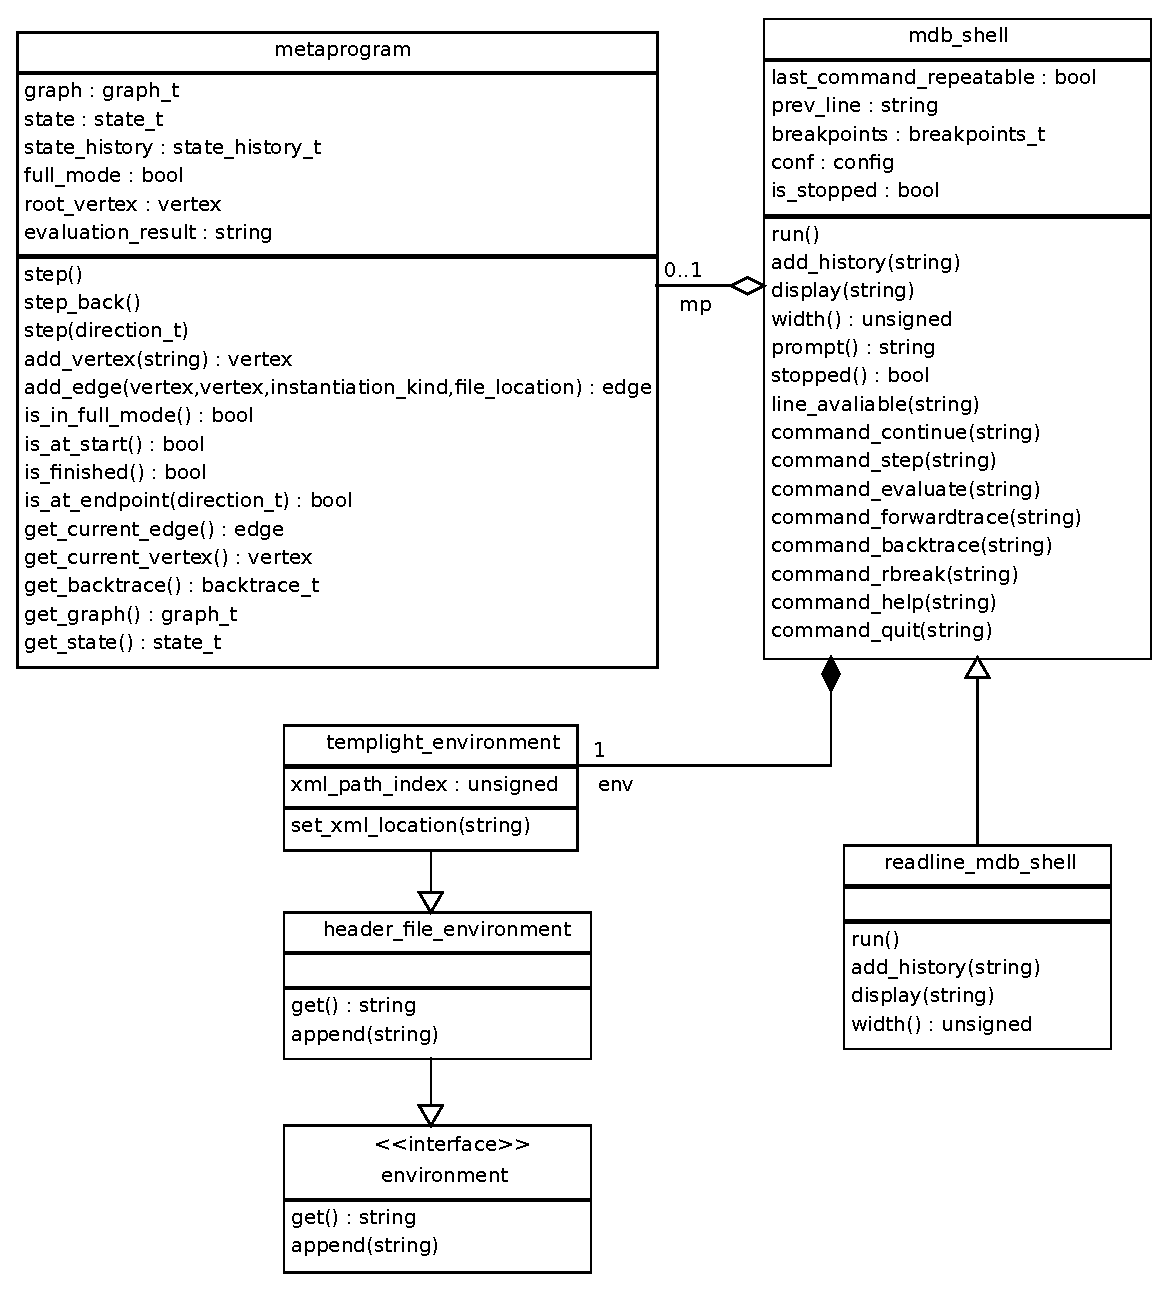
\includegraphics[width=\textwidth]{img/mdb_class_diagram.eps}
\end{figure}

Notes:
\begin{itemize}
    \item
        Only public member functions and private member variables are shown
        on the diagram.
    \item
        Lot of smaller, helper structures and classes are hidden.
    \item
        There is another class inheriting \texttt{mdb\_shell} called
        \texttt{mdb\_test\_shell}. This class is only used for testing
        purposes to mock out the actual shell and Readline related
        functionalities, which would make automated testing very difficult.
\end{itemize}

\section{Libraries used}

Several libraries are used by Metadebugger. In the section the main libraries
are listed.

\subsection{Boost\cite{boost}}

Boost is a set of open source C++ libraries that provide ready to use solutions
to common tasks. In Metadebugger several Boost libraries are being used:
\begin{description}
    \item[Boost.Graph] \hfill \\
        This library provides a generic interface and implementations of graph
        data-structures and algorithms.

        In Metadebugger the information which is gathered by Templight is
        stored in a Boost.Graph data-structure. Since the whole program is
        revolving around the metaprogram which being debugged, it was very
        important to choose a robust and flexible graph library.
    \item[Boost.Optional] \hfill \\
        Unlike in some programming languages, in C++ stack allocated objects
        cannot have a null value. This have some advantages, for example the
        programmer doesn't have to check for a null value before doing
        operations on an object.

        But at the same time, sometimes it is useful to have an object state,
        in which the object is invalid in purpose. Boost.Optional provides an
        easy way to turn any type into a type which can have an invalid state
        called \verb|boost::none|.
    \item[Boost.PropertyTree] \hfill \\
        The Boost.PropertyTree library provides a data structure that stores an
        arbitrarily deeply nested tree of values, indexed at each level by some
        key.

        Metadebugger makes use of the xml parsing capabilites of
        Boost.PropertyTree to parse the xml created by Templight.
    \item[Boost.Regex] \hfill \\
        Boost.Regex provides support for regular expressions in C++.

        Metadebugger uses regular expressions to match type names when
        breakpoints are used.
    \item[Boost.Filesystem] \hfill \\
        Boost.Filesystem provides cross platform solutions to manipulate the
        file system.

        Metadebugger uses Boost.Filesystem to create and delete the temporary
        file where the output of Templight is stored until it's processed.
    \item[Boost.StringAlgorithm] \hfill \\
        Boost.StringAlgorithm provides a handful of useful string-related
        algorithms.

        Metadebugger has to manipulate strings in various contexts and makes
        use of a few algorithms contained in this library.
    \item[Boost.LexicalCast] \hfill \\
        Boost.LexicalCast provides an easy way to convert numbers to string
        form and the other way around.

        Metadebugger uses this library during parsing of the Templight xml
        file.

\end{description}

\subsection{Just\cite{just}}

Just is a collection of lightweight C++ libraries developed by Sinkovics. The
following Just libraries are used in Metadebugger:
\begin{description}
    \item[just::console] \hfill \\
        The just::console library provides a cross platform interface to output
        colored text to a console interface.

        Metadebugger uses colored text in its output for easier readability.
    \item[just::test] \hfill \\
        Just::test is a testing library.

        Metadebugger uses just::test to create unit and integration test cases.
\end{description}

\subsection{Clang\cite{clang}}

Clang is a C++ frontend for LLVM. Together they form a highly customizable C++
compiler. Clang is used to compile the source code given as an input to
Metadebugger.

\subsection{Templight\cite{templight}}

Templight (in its current form) is a source code patch to Clang. With
Templight, Clang is able to generate output about the template instantiation
steps during compilation. Metadebugger takes this output and creates the
necesseary data structures to be able to simulate the compilation.

\subsection{Readline\cite{readline}}

The Readline library is the de facto standard library used to handle user
inputs in software that uses an interactive command line interface.

